\section{Initial issues with implementation}
After establishing a clear direction for the project, implementation could begin.
However, the GIRAF project ran into certain difficulties in the beginning of sprint 1 implementation.
This section details the biggest problems encountered.

\subsection{Change of framework}\label{change-of-framework}
The developers of last year had made the choice of changing the development framework from using Android Studio to Xamarin in order to support building the application for iOS.
However, with the introduction of full stack teams this lead to a series of issues. Approximately 1/4th of the developers on the GIRAF project this year were using some variation of Linux as their operating system of choice, which Xamarin does not officially support.
Previously, this had not been a problem, as only the dedicated front-end development group would be working with Xamarin. 
Only the people in this group would need to be on Windows or MacOS in order to compile the front-end part of the application.
With full stack groups, more or less every group would be affected by this problem, having group members who could not compile the front-end of the application.
\\\\
This led to one group spending a lot of time investigating different ways to make the Xamarin project compile on Linux, but as time progressed it was deemed infeasible to implement a series of workarounds to make the project compile.
Some people got Xamarin to compile on Linux, but it seemed that the processes and methods necessary to make Xamarin compile were not identical to other versions of Linux.
Instead, the front-end skill group held a meeting to discuss the pros and cons of making the Xamarin project work versus changing to another framework, which would natively support Linux.
During the meeting, a series of pros and cons for changing the framework were worked out:

\begin{itemize}
    \item [\textbf{Pros}]
    \item The most difficult part to reimplement is authorization
    \item It is difficult to maintain the Linux compatibility for Xamarin, as the problems varied between machines
    \item The \texttt{Swagger API} generates bad code, which can be fixed while changing the framework
    \item It would be possible to implement a cleaner UI while re-working the front-end
    \item It will be easier for future students to work on GIRAF if it works on Linux
    \item [\textbf{Cons}]
    \item Changing will require a new language that the developers may not have worked with before
    \item Some people have managed to get Xamarin to compile
    \item It is possible to compile Xamarin using Windows, which is offered for free by the university
    \item It will increase the time that is spent before a product can be released to the customers
\end{itemize}
\noindent
After discussing the pros and cons internally in the skill group, all the developers on the GIRAF project were invited to an open discussion. 
This discussion was held to hear the input of people who were not in the front-end skill group, as it felt like a decision that was too big to make without consulting everyone.
After the open meeting, it was clear that the majority of the developers were ready to make the change, and it was decided that \texttt{Flutter} would be used as a new framework. 
\\\\
\texttt{Flutter} is an open-source mobile application development framework by Google, that uses the \texttt{Dart} language.
One of the major reasons for choosing Flutter over alternative frameworks such as \texttt{React Native} or \texttt{Ionic} is the availability of tutorials and guides, for both Flutter and Dart. 
Likewise, it was deemed that, due to Flutter being developed by Google, the chance that it would become outdated anytime soon was highly unlikely.
In order to ease the transition from Xamarin to Flutter, a Flutter team was assembled.
This team was assigned the task of spending the upcoming weekend setting up the base of the Flutter project, and to help the other students get started by running a Flutter workshop in the following week.

\subsubsection{Flutter weekend}
To make the transition to Flutter from Xamarin smoother for everyone in the GIRAF project, a group of volunteers were assembled that spent the following weekend laying the ground work for switching to Flutter. 
The team spent the weekend implementing the core part of the application, so that the rest of the groups in the GIRAF project had something to work from. 
The team consisted of eight people, where four of them were from group sw611f19, two from the PO group, one from group sw612f19 and one from the process group.
The weekend was spent implementing the API in Flutter, re-creating all the models on the frontend part of the application and implementing a simple graphical user interface for the application.
\\\\
Previously, when the application was implemented in Xamarin, they had made use of Swagger to automatically generate the API for the application's frontend.
This did not work optimally, due to faulty code generation from Swagger, and the team decided to implement it manually instead, to ensure that it worked as intended.
\\\\
A base design of the login screen, the week plan screen and the settings screen were created to get some insight into how applications are designed in Flutter, and to serve as a foundation such that the rest of the groups had some examples to look at when they were to implement user stories in the coming week.
A big part of the weekend was also spent looking at best practices and standards regarding Flutter development, and which architectures could be used when implementing the application.
The team settled on using the \texttt{BLoC} structure and some ground work was done to facilitate this, and an example \texttt{BLoC} was implemented as an example of what a \texttt{BLoC} should look like.
The PO group created new user stories that focused on implementing the whole application from scratch and getting the application to the same state it was in before the change of framework.
\todo{Overvej at flytte flutter introduction fra implementation herop. Mangler noget forklaring på bloc osv.}
\\\\
The following Monday, one of the group members of group sw611f19 assisted the product owners in writing more technical descriptions of the user stories that were to be implemented in the following week, to make it easier for the groups who did not participate in the weekend to get started with the development relating to their user stories.
A workshop was held on the following day for all the groups in the GIRAF project, where a brief introduction of Flutter was given, and some live coding was done to give an example of the workflow in Flutter.
At the workshop, all groups were then assigned user stories that they could start to work on.

\subsection{New user stories}
This section details the user stories that were created and deemed of highest importance following the change of framework.
These user stories were created with the purpose of reimplementing the foundation of the program, making it usable by customers once again.
In contrast to the initial sprint planning, we also decided to assign user stories to our group.
This choice was made as many of our initial PO responsibilities had been handled, and we could help attain the required basic functionality as fast as possible.
All assigned user stories and the groups working to implement them can be seen on \autoref{table:user-stories-sprint-1}.
\begin{table}[H]
    \begin{tabular}{|p{2.8cm}|p{8cm}|p{1.6cm}|}
    \hline
    Issue ID        & User story name                                                                                                                                                          & Group assigned       \\ \hline
    Weekplanner\#23 & As a guardian I would like to be able to access parts of the system through the top bar so that I can easily go to the screen I want & Group 2            \\ \hline
    Weekplanner\#43 & As a guardian I would like to be able to view a given citizens week plan so that I can get an overview of what is happening this week for them & Group 10             \\ \hline
    Weekplanner\#44 & As a citizen I would like to be able to view my week plan so that I know what is going to happen & Group 10               \\ \hline
    Weekplanner\#46 & As a guardian I would like to be able to search for pictograms when adding a new activity so that I can find a pictogram that suits the activity & Group 11              \\ \hline
    Weekplanner\#47 & As a guardian I would like to be able to choose a citizen so that I can choose who I’m editing the week plan for  & Group 9             \\ \hline
    Weekplanner\#48 & As a guardian I would like to be able to log into the system using a username and password, so that I can see my associated citizens & Group 9             \\ \hline
    Weekplanner\#49 & As a guardian I would like to be able to log out so that the system is not left logged in after I’m done using it. & Group 12              \\ \hline
    Weekplanner\#50 & As a guardian I would like to be able to choose which week plan to show the citizen so that I can have multiple plans available to each citizen & Group 13             \\ \hline
    Weekplanner\#51 & As a guardian I would like to be able to create a new week plan so that it is suited to the given citizens week & Group 8             \\ \hline
    \end{tabular}
    \caption{User stories for all groups in sprint 1 after changing to flutter.}\label{table:user-stories-sprint-1}
\end{table}
\noindent
We are group 10, and were assigned the user stories \textit{Weekplaner\#43} and \textit{Weekplanner\#44}.
These user stories involved the weekplanner screens for both the guardian and the citizen modes.

\subsection{New design guide}
As Xamarin was changed to Flutter, the entire frontend had to be reworked. 
Therefore we took a look at the old design guide and decided that there were things we wanted to changed in order to get a more modern and simple design.
This meant that a new design guide had to be created.
The first thing we wanted to do was make the design guide more compact.
The old design guide was an 80 pages long pdf file that could be downloaded from Phabricator.
The new design guide is instead found on the GitHub wiki alongside the rest of the GIRAF project, making it easier to find the guide and the sections that a developer would need.
As seen on \autoref{fig:designguides}, the new one has a smaller table of contents.
The old guide had 4 pages of content in the PDF file.
The reason that the new design guide is so much smaller, is mostly that a lot of the content in the old guide was specifically about Android Studio implementation details.
This is not relevant for the project development in Flutter, as it natively encourages following the material design guidelines.
However, the new design guide will most likely grow larger as the project goes on, but this should be an easy task for future students now that it is available as markdown files rather than a pdf document without any source. 

\begin{figure}[H]
    \begin{subfigure}{0.5\textwidth}
    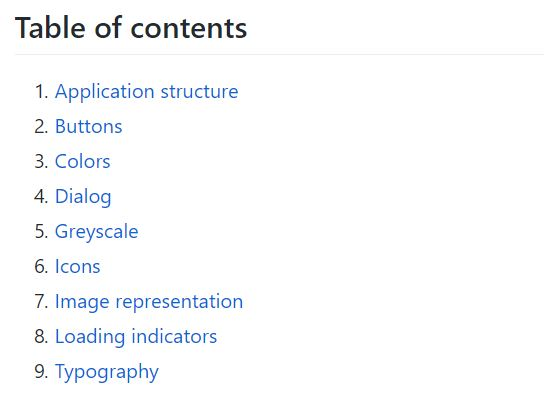
\includegraphics[width=1\linewidth, height=5cm]{figures/table-of-content-designguide.JPG}
    \caption{The table of contents for the new design guide.}
    \label{fig:new-designguide}
    \end{subfigure}
    \begin{subfigure}{0.6\textwidth}
        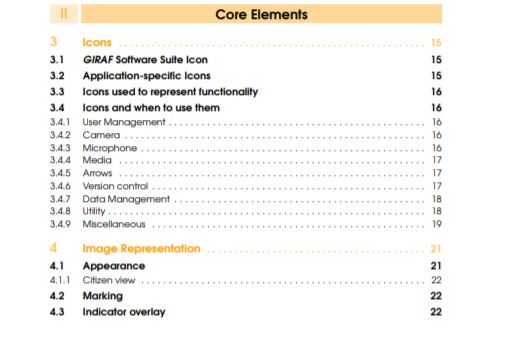
\includegraphics[width=1\linewidth, height=5cm]{figures/old-design-guide}
    \caption{Excerpt of the old design guide contents. Continues for another 3 pages}
    \label{fig:old-designguide}
    \end{subfigure} 
    \caption{New and old design guide.}
    \label{fig:designguides}
\end{figure} 

\subsubsection{Colors}
For the colors in GIRAF not much has changed from the old design guide to the new one. 
The only thing that changed was the colors for the weekdays.
The new colors are more dull compared to the old colors, giving a more subdued look with a more gentle impression.

\subsubsection{Typography}
The standard text color for typography is black.
The font was changed to \textit{Quicksand font}, because the customers prefer the letter "a" to be the handwritten version which this font allows.
The size of the font is 30 pt in portrait mode and in landscape mode it is 20 pt.
The text should also never be bold, italic or underlined to ensure consistent design.
\todo{Confirm lige skriftstørrelser. Stemmer ikke overens med design guide nu.}

\subsubsection{Icons}
Every icon in the old design guide has been changed for the new design guide.
The old icons had an out of date look, and did not result in a good design for the application.
Most of the icons that are used in this project are icons from the \textit{Font Awesome} project, which is a font and CSS framework.
These are easy to import in \texttt{Flutter}, and by using the icons in the same package the application is more consistent and will give the users a better experience, as they know the icons throughout the program.
Three custom icons needed to be created. \\
These can be seen on \autoref{fig:change-profile-icons}. \\\\
These icons are used for switching from guardian to citizen and vice versa and a new add timer icon.
In the old design guide there was only one icon for switching between guardian and citizen.
We wanted to make it more obvious which mode the user is in and decided to have two icons, one for each switch.
Depending on the mode the user is in the corresponding silhouette is colored in green.

\begin{figure}[htp]

    \centering
    
\includegraphics[width=.1\textwidth]{figures/changeToGuardian}\hfill
    
\includegraphics[width=.1\textwidth]{figures/changeToCitizen}\hfill
    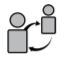
\includegraphics[width=.1\textwidth]{figures/old-change-profile}
    
    \caption{ The leftmost icon is to change from citizen to guardian. The middle icon is the one to change from guardian to citizen and the rightmost icon is the old icon for changing profile.}
    \label{fig:change-profile-icons}
\end{figure}


